{\documentclass[sigplan, screen]{acmart}
\usepackage[german, main=ngerman]{babel}
\usepackage{fancyhdr}
\usepackage{listings, lstautogobble}
\usepackage{tablefootnote}

\def\sectionautorefname{Abschnitt}
\def\subsectionautorefname{Abschnitt}
\def\subsubsectionautorefname{Abschnitt}
\def\tableautorefname{Tabelle}
\def\figureautorefname{Figur}
\def\lstlistingautorefname{Listing}

\AtBeginDocument{%
  \providecommand\BibTeX{{%
    \normalfont B\kern-0.5em{\scshape i\kern-0.25em b}\kern-0.8em\TeX}}}

\definecolor{backcolour}{rgb}{0.95,0.95,0.92}
\definecolor{lightgray}{rgb}{.9,.9,.9}
\definecolor{darkgray}{rgb}{.4,.4,.4}
\definecolor{purple}{rgb}{0.65, 0.12, 0.82}
\definecolor{lightgreen}{rgb}{0.45, 0.8, 0.45}

\lstdefinelanguage{JavaScript}{
  keywords={break, case, catch, continue, debugger, default, delete, do, else, false, finally, for, function, if, in, instanceof, new, null, return, switch, this, throw, true, try, typeof, var, void, while, with},
  keywordstyle=\color{purple}\bfseries,
  ndkeywords={type, class, export, boolean, throw, implements, import, this},
  ndkeywordstyle=\color{darkgray}\bfseries,
  identifierstyle=\color{black},
  sensitive=false,
  comment=[l]{//},
  morecomment=[s]{/*}{*/},
  commentstyle=\color{gray}\ttfamily,
  stringstyle=\color{lightgreen}\ttfamily,
  morestring=[b]',
  morestring=[b]"
}

\lstdefinestyle{mystyle}{
  language=JavaScript,
  basicstyle=\ttfamily\footnotesize,
  breakatwhitespace=false,         
  breaklines=true,                     
  keepspaces=true,                 
  numbers=left,                    
  numbersep=5pt,                  
  showspaces=false,                
  showstringspaces=false,
  showtabs=false,                  
  tabsize=2,
  autogobble=true,
  frame=single,
  columns=flexible
}

\lstset{style=mystyle}

\makeatletter
\newlength{\singlespace}
\newlength{\gobble}
\newlength{\numbersep}
% The width of a single space.
\settowidth{\singlespace}{\lst@basicstyle \ }
\setlength{\singlespace}{-\singlespace}

\lst@Key{firstlineandnumber}\relax{\def\lst@firstline{#1\relax}\def\lst@firstnumber{#1\relax}}
\makeatother

\setcopyright{none}
\settopmatter{printacmref=false, printfolios=true}
\renewcommand\footnotetextcopyrightpermission[1]{}
\copyrightyear{2022}
\acmYear{2022}

\acmBooktitle{Hauptseminar II WiSe 22/23, gehalten von Kevin Linne, M.Sc.}

\begin{document}

\title{Möglichkeiten zur asynchronen Kommunikation zwischen Webbrowser und Server}

\author{Hendrik Wagner}
\email{hendrik.wagner@mni.thm.de}

\affiliation{%
  \institution{Technische Hochschule Mittelhessen}
  \streetaddress{Wiesenstraße 14}
  \city{Gießen}
  \state{Hessen}
  \postcode{35390}
  \country{Germany}
}

\begin{abstract}
  Bei Webseiten und Webapplikationen ist es häufig notwendig, dass der Server Daten an den Client (Webbrowser) sendet, ohne dass dieser eine Anfrage dafür gestellt hat.
  Dies ist gemäß der HTTP-Spezifikation nicht vorgesehen, weshalb eine Reihe von alternativen Methoden entwickelt wurden, um diese Funktionalität zu ermöglichen.

  In diesem Artikel die Methoden \emph{Polling}, \emph{Long-Polling}, \emph{Streaming} und \emph{WebSockets} vorgestellt und verglichen.
  Dabei wird auf die Funktionsweise, die Implementierung und die Vor- und Nachteile eingegangen.
\end{abstract}

\keywords{web, http, WebSockets, polling, bidirectional communication, asynchronous communication}

\maketitle
\lhead{\small Möglichkeiten zur asynchronen Kommunikation zwischen Webbrowser und Server}
\rhead{\small Hendrik Wagner}

\tableofcontents
\newpage

% Möglichkeiten für Client-Server Kommunikation nach Aufruf einer Website
% Auseinandersetzung mit...
% - Was sind und wie funktionieren Websockets (Spezifikation), Polling, Long Polling ✔️
% - Realisierungen (insb. Serverside-Setup von Websockets, ggf. Polling-Algorithmen)  ✔️
% - Vergleich von manuell implementierten Websockets, Polling (Auch mit Blick auf Performance, TCP packets) ✔️

% - Vergleich/Analyse von existierenden Websocket-Frameworks
% - statistiken (verbreitung, wie wirds eingesetzt) ✔️
% - umsetzung von ws durch aktuelle frameworks, was machen die, welche frameworks gibt es
% - spezifikation von ws ✔️

\section{Einleitung}

Moderne Webapplikationen sind in der Regel auf eine bidirektionale Kommunikation zwischen Client und Server angewiesen,
um zum Beispiel Benachrichtigungen oder Echtzeitdaten anzuzeigen.
Webseiten basieren in der Regel auf dem HTTP-Protokoll, nach welchem alle Anfragen vom Client initiiert werden müssen.
Um also eine asynchrone Kommunikation zwischen Client und Server zu ermöglichen, muss entschieden werden, wie mit dieser Einschränkung umgegangen werden soll.

Diese Arbeit beschäftigt sich mit verschiedenen Ansätzen zur asynchronen Kommunikation zwischen Client und Server.
Sie soll dabei helfen, die Vor- und Nachteile der einzelnen Methoden zu verstehen und eine Entscheidungshilfe für die Wahl der geeigneten Methode liefern.

Dabei wird auf klassisches Polling, die Polling-Varianten \emph{Long Polling} und \emph{Streaming}, sowie auf die bidirektionale Kommunikation mittels \emph{WebSockets} eingegangen.
Es wird jeweils die Funktionsweise der Methoden erläutert, eine Beispielimplementierung vorgestellt und die Vor- und Nachteile der einzelnen Methoden aufgezeigt.
Dabei werden Performance und Implementierungsaufwand berücksichtigt.

Zunächst wird die theoretische Funktionsweise der einzelnen Methoden erläutert.
Es wird dafür auf die Spezifikationen der einzelnen Methoden sowie exemplarische Nachrichtensequenzen zurückgegriffen.
Anschließend wird mit jeder Methode eine Chatanwendung implementiert, um die Funktionsweise zu demonstrieren.
Anhand der Implementierung wird die Implementierungsaufwand und die Performance der einzelnen Methoden verglichen.
Abschließend werden die Vor- und Nachteile der einzelnen Methoden aufgezeigt.
Zudem werden gängige Frameworks kurz vorgestellt und mit den implementierten Methoden verglichen.
Zuletzt werden die Ergebnisse zusammengefasst und eine Empfehlung für die Wahl der geeigneten Methode gegeben.

% - grund für die arbeit
% - was wird behandelt, was nicht
% - wie ist die methodik, was wird gemacht, was nicht

\section{Vorstellung der Kommunikationsvarianten}

Es gibt eine Reihe von Ansätzen, wie eine bidirektionale Kommunikation zwischen Client und Server im Web realisiert werden kann.
In diesem Abschnitt werden die wichtigsten Ansätze chronologisch vorgestellt und kurz erläutert.

\subsection{Klassisches Polling}

Unter dem 1990 eingeführten \cite[Abs. 1.2]{fielding_http_2022} HTTP-Protokoll gibt es eine Reihe von Anfragen, die der Client an den Server senden kann \cite{noauthor_http_nodate}.
Das Protokoll definiert dabei explizit einen Client (in unserem Fall der Browser), welcher Anfragen an den Server (Bereitstellender der Webinhalte) versendet.
Dieser wartet auf Anfragen und beantwortet diese \cite[Abs. 1.3]{fielding_http_2022}.

Für das Vorhaben sind GET-Requests besonders relevant, also klassische Abfragen von Inhalten mittels HTTP.
Polling, in diesem Anwendungsfall wohl am besten übersetzt mit \emph{zyklische Absuche} oder \emph{Sendeaufruf},
beschreibt in der Webentwicklung das regelmäßige Abrufen (in einem Intervall $\Delta t$) von neuen Inhalten.
Abhängig von der Implementierung gilt das Intervall entweder ab dem Zeitpunkt des letzten Abrufs oder ab dem Zeitpunkt der letzten Antwort des Servers.
Gibt es Nachrichten, die der Server bereitstellen möchte, beantwortet dieser die Anfrage mit den neuen Inhalten --
andernfalls wird der Antwortkörper leer sein.

\begin{figure}
  \centering
  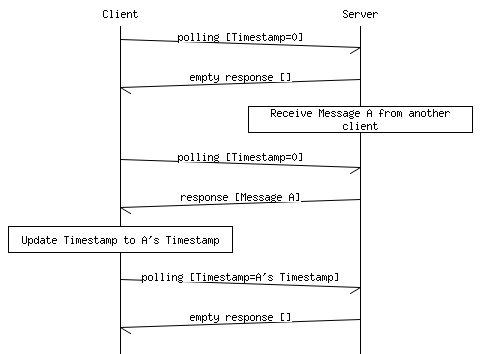
\includegraphics[width=.45\textwidth]{assets/msc/polling.png}
  \caption[Nachrichtenempfang bei Polling-Kommunikation]{Beispiel von Nachrichtenempfang bei klassischem Polling.
    Der Client sendet regelmäßig eine Anfrage an den Server, welche entweder mit leerer Antwort oder mit neuen Inhalten beantwortet wird.
    Die Länge der Zeitspanne $\Delta t$ zwischen zwei Polling-Anfragen ist implementierungsabhängig.}
  \label{fig:polling}
\end{figure}

\begin{figure}
  \centering
  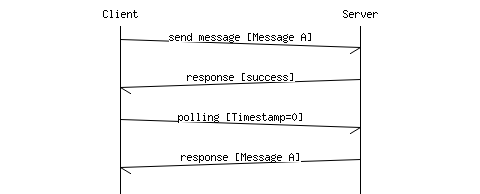
\includegraphics[width=.45\textwidth]{assets/msc/polling-send.png}
  \caption[Nachrichtenversand bei Polling-Kommunikation]{Beispiel von Nachrichtenversand bei klassischem Polling.
    Der Client sendet eine Nachricht an den Server, welche daraufhin mittels Polling abgerufen werden kann.}
  \label{fig:polling_send}
\end{figure}

\subsubsection{Spezifikation}
\label{sec:polling-spec}

Polling ist in der Spezifikation von HTTP nicht definiert, es handelt sich hierbei um eine Implementierung des Clients und des Servers.
Meist wird Polling durch JavaScript-Code realisiert, welcher in einem bestimmten Intervall (z. B. alle 5 Sekunden) eine Anfrage an den Server sendet.
Diese Anfrage ist ein GET-Request, welcher die URL der Anwendung enthält.
Wie der Server auf diese Anfrage antwortet, ist Implementierungsabhängig:
So könnte er zum Beispiel den gesamten abgefragten Inhalt bei jeder Anfrage übermitteln, oder nur Änderungen, die dieser Client noch nicht übermittelt bekommen hat.
Eine solche Optimierung setzt allerdings voraus, dass der Server in der Lage ist, zu identifizieren, welche Änderungen der Client bereits erhalten hat.

\subsection{Long Polling}

Eine Optimierung des Polling-Konzepts ist das sog. \emph{Long Polling}.
Dabei wird die Antwort auf eine HTTP-Anfrage zurückgehalten, bis der Server eine Nachricht versenden will \cite{noauthor_long_2021}.

\begin{figure}
  \centering
  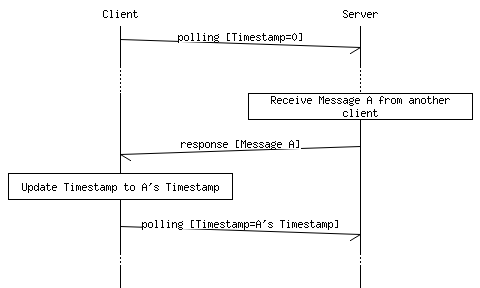
\includegraphics[width=.45\textwidth]{assets/msc/long-polling.png}
  \caption[Nachrichtenempfang bei Long Polling]{Beispiel von Nachrichtenempfang bei Long Polling.
    Der Server beantwortet die Anfrage des Clients erst, wenn er eine Nachricht hat, die er übermitteln möchte.
    Der Nachrichtenversand verläuft analog zu Polling.}
  \label{fig:long_polling}
\end{figure}

\subsection{Streaming}

Eine weitere Optimierung des Polling-Konzepts ist das sog. \emph{Streaming}, manchmal auch \emph{Comet} oder \emph{Server Push} genannt.
Es verwendet die HTTP Transferkodierung Chunking (vgl. \cite[Abs. 7.1]{fielding_http_2022}),
also dem Aufspalten der Antwort in mehrere Packets, in welchen dann einzelne Nachrichten versendet werden.
So kann die Anzahl an Anfragen ausgehend vom Client an den Server auf eine reduziert werden --
der Server terminiert nie die Antwort auf die erste Anfrage \cite[Abs. 3]{saint-andre_known_2011}.

\begin{figure}
  \centering
  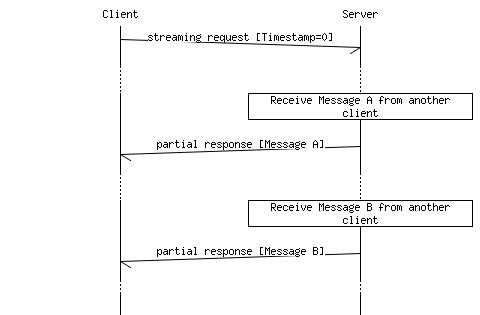
\includegraphics[width=.45\textwidth]{assets/msc/streaming.png}
  \caption[Nachrichtenempfang bei Streaming]{Beispiel von Nachrichtenempfang bei Streaming.
    Der Client initiiert den Streaming-Prozess durch eine einmalige Anfrage.
    Daraufhin sendet der Server Teilantworten an den Client, sobald neue Nachrichten verfügbar sind.
    Der Nachrichtenversand verläuft analog zu Polling.}
  \label{fig:streaming}
\end{figure}

\subsection{WebSockets}

WebSockets sind ein vom IETF\footnote{Internet Engineering Task Force.} entwickeltes Protokoll,
welches 2011 als Standard veröffentlicht wurde \cite{melnikov_websocket_2011}.
Grund für dessen Entstehung ist unter anderem die Erkenntnis, dass der Versuch, HTTP zu verwenden,
um bidirektionale Kommunikation zu ermöglichen, vermeidbare Komplexität und Ineffizienz mit sich bringt \cite[S. 137f]{lubbers_pro_2010}.

Es handelt sich bei WebSockets um ein vollwertiges Protokoll, welches auf TCP aufbaut.
Es versucht, die Probleme von Polling, Long Polling und Streaming direkt zu adressieren (vgl. \cite[Abs. 1.1]{melnikov_websocket_2011}),
indem es eine TCP-nahe Verbdingung zwischen Client und Server aufbaut und unterstützt.

Genauer baut WebSockets einen Tunnel zwischen TCP und IP auf, sodass darauffolgend TCP-Kommunikation systemübergreifend erfolgen kann (vgl. \cite[Abs. 1.5]{melnikov_websocket_2011}).
HTTP wird dann lediglich für die initialen Handshakes verwendet -- danach nicht mehr.

\begin{figure}
  \centering
  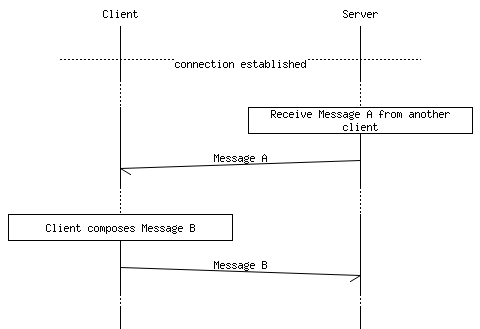
\includegraphics[width=.45\textwidth]{assets/msc/websockets.png}
  \caption[Nachrichtenaustausch bei WebSockets]{Beispiel von Nachrichtenaustausch bei WebSockets.
    Nach dem Handshake wird eine TCP-Verbindung zwischen Client und Server aufgebaut.
    Von nun an können Nachrichten in beide Richtungen ausgetauscht werden.}
  \label{fig:websockets}
\end{figure}

\subsubsection{Spezifikation}
\label{sec:websocket-spec}
Um eine Verbindung über einen WebSocker aufzubauen, wird zunächst vom Client aus eine HTTP-Anfrage gesendet.
Gemäß der Spezifikation muss es sich hierbei um eine GET-Request an den Pfad, auf dem der WebSocket hinterlegt ist, handeln.

Wäre die WebSocket URI \texttt{ws://example.org/chat}, so wäre die erste Zeile der HTTP-Anfrage \texttt{GET /chat HTTP/1.1} \cite[Abs. 4.1]{melnikov_websocket_2011}.
Zusätzlich müssen in der Anfrage unter anderem der Host (hier \texttt{Host: example.org}) und die Intention (Felder \texttt{Connection: Upgrade} und \texttt{Upgrade: websocket}) als Headerfelder übermittelt werden.

Der Server antwortet auf diese Anfrage mit einer HTTP-Response, welche entweder den Statuscode 101 \emph{Switching Protocols} oder einen Fehlercode enthält.
Zudem meldet er bei erfolgreichem Protokollwechsel die vom Client angegebene Intention zurück.

Wurde die Verbindung vom Server akzeptiert, können nun Client und Server direkt miteinander kommunizieren.
Für die Datenübermittlung sieht das WebSocket Protokoll eine auch in anderen Protokollen ähnlich vertretenes Frame-System vor,
also dem Versenden von Daten in Form von Frames, welche jeweils einen Header und eine Payload enthalten.
Header enthalten u. A. den Opcode\footnote{Opcodes (\emph{Operation Codes}, dt. \emph{Befehlscode}) können bei WebSockets Frames mit Text- oder Binärdaten ankündigen, eine vorherige Frame fortsetzen, die Verbindung schließen, oder einen Ping/Pong markieren.} und die Payload-Länge (vgl. \cite[Abs. 5.2]{melnikov_websocket_2011}).

\section{Beispielhafte Implementierungen}

Um die Unterschiede zwischen den Kommunikationsvarianten ersichtlich zu machen, werden diese für eine Chat-Applikation implementiert.
Dabei wird jeweils auf die Client- und Serverseitige Implementierung eingegangen.

Die Realisierung erfolgt in TypeScript, wobei die Serverseitige Implementierung auf Node.js basiert.
Der Client benutzt das Vue.js-Framework mit Vuetify, um die Darstellung zu vereinfachen.
Implementierungen in anderen Frontend-Frameworks erfolgen analog.
Es wird nicht auf die Darstellung der Nachrichten oder des Chats eingegangen, da dies nicht relevant für die Implementierung ist.
Entsprechende Codeabschnitte sind daher ausgelassen.

Die vollständige Implementierung der Frontendkomponenten ist im Repository im Verzeichnis \\\cite[\texttt{code/client/src/components/}]{wagner_seminar2022_2022} zu finden.
Der gesamte Code für alle Serverkomponenten befindet sich in \cite[\texttt{code/server/chatserver.ts}]{wagner_seminar2022_2022}.

\subsection{Implementierung von Polling}

Für alle Arten von Polling verwaltet der Server eine Liste aller bisher empfangenen Nachrichten.
Neue von einem Client übermittelte Nachrichten werden mit Autor, Zeitstempel und Text in diese Liste eingefügt.

\begin{lstlisting}[caption={Beispielhafte \emph{Message}}, label={lst:message-json}, numbers=none]
{
  content: "Hello World!",
  sender: "Alice",
  timestamp: "2022-12-04T19:29:13.455Z"
}
\end{lstlisting}

Im Falle des klassischen Polling wird der Client in regelmäßigen Zeitabständen (hier $\Delta t = 2s$) eine Anfrage an den Server senden, um neue Nachrichten abzufragen.
Dementsprechend muss der Server seine Nachrichtenliste nach für den Client neuen Nachrichten filtern und diese zurückgeben.

\subsubsection{Polling Server}

Der Server besteht aus einer Instanz von \texttt{http.Server}, welche die HTTP-Anfragen \texttt{/polling} und \texttt{/polling/send} verarbeitet.
Zudem verwaltet er ein Array mit allen Nachrichten, die bisher gesendet wurden.

Bei einer Anfrage an \texttt{/polling} wird mit einem Zeitstempel gearbeitet,
sodass der Server nur die Nachrichten zurückgibt, die nach diesem Zeitstempel eingegangen sind.
Da die Abfragen nach Nachrichten in der Regel öfter als die Nachrichten selbst gesendet werden,
wird das Array der Nachrichten oft leer sein.

\lstinputlisting[caption={Polling Server: Nachrichtenabfrage}, label={lst:polling-server-polling}, firstlineandnumber=37, lastline=40]{../code/server/chatserver.ts}

Im Falle einer Anfrage an \texttt{/polling/send} wird die Nachricht in das Array eingefügt und der Client mit dem Statuscode 200 \emph{OK} bestätigt.

\lstinputlisting[caption={Polling Server: Nachrichtenempfang}, label={lst:polling-server-send-message}, firstlineandnumber=41, lastline=45]{../code/server/chatserver.ts}

\subsubsection{Polling Client}

Der Client besteht aus der Komponente \texttt{PollingChat.vue}, welche die Funktionen zum Senden und Empfangen von Nachrichten enthält.
Die Darstellung, sowie die Speicherung von Nachrichten und Nutzdaten erfolgt in der Komponente \texttt{ChatPage.vue} (vgl. jeweils \cite[\texttt{code/client/src/components/}]{wagner_seminar2022_2022}).

Um eine Nachricht zu versenden, wird lediglich eine HTTP POST-Anfrage an die URL \texttt{/polling/send} gesendet.
Die Nachricht wird dabei als JSON-Objekt in der Anfrage übermittelt.

\lstinputlisting[caption={Polling Client: Nachrichtenversand}, label={lst:polling-client-send-messages}, firstlineandnumber=14, lastline=22]{../code/client/src/components/PollingChat.vue}

Mittels einer HTTP POST-Anfrage an die URL \texttt{/polling} werden die Nachrichten abgefragt\footnote{Hier unterscheidet sich die Implementierung von der Spezifikation in \autoref{sec:polling-spec}. Der Zeitstempel hätte ebenfalls als Parameter übermittelt werden können.}.
Die Anfrage enthält dabei den Zeitstempel der letzten Nachricht, die der Client erhalten hat, als String.
Der Server antwortet mit einer Liste von Nachrichten, die nach diesem Zeitstempel eingegangen sind.
Diese werden anschließend an die Komponente \texttt{ChatPage.vue} mittels des Events \texttt{appendMessages} übermittelt.

Um die Nachrichten regelmäßig abzufragen, wird ein Intervall gesetzt, welches alle zwei Sekunden die Funktion \texttt{fetchMessages} aufruft.
Dieses Intervall wird bei der Initialisierung der Komponente gesetzt und bei der Entfernung der Komponente wieder gelöscht.

\lstinputlisting[caption={Polling Client: Nachrichtenabfrage}, label={lst:polling-client-get-messages}, firstlineandnumber=24, lastline=44]{../code/client/src/components/PollingChat.vue}

\subsection{Implementierung von Long Polling}

Die Implementierung von Long Polling ist sehr ähnlich zu der von Polling.
Die einzige Änderung ist, dass der Server die Anfrage nicht sofort beendet, sondern die Verbindung offen hält, bis eine neue Nachricht eingegangen ist.
Dazu wird sowohl der Client als auch der Server angepasst.

\subsubsection{Long Polling Server}

Der Server verwaltet nun eine Menge von offenen Verbindungen.
Geht eine Anfrage ein, wird diese entweder mit neuen Nachrichten beantwortet, oder die Verbindung wird in die Menge der offenen Verbindungen aufgenommen.

\lstinputlisting[caption={Long Polling Server: Nachrichtenabfrage}, label={lst:long-polling-server-get-messages}, firstlineandnumber=67, lastline=76]{../code/server/chatserver.ts}

Geht eine neue Nachricht ein, wird diese an alle bis dahin erhaltenen offenen Verbindungen gesendet.
Dadurch werden alle offenen Verbindungen geschlossen.

Aufgrund von asynchroner Bearbeitung der Anfragen kann es hier zu Race-Conditions kommen.
Daher wird der Versuch, Nachrichten an gespeicherte Verbindungen zu versenden, in einem try-catch-Block abgefangen und Errors ignoriert.

\lstinputlisting[caption={Long Polling Server: Nachrichtenempfang}, label={lst:long-polling-server-send-messages}, firstlineandnumber=77, lastline=94]{../code/server/chatserver.ts}

\subsubsection{Long Polling Client}

Der Client ändert sich ebenfalls nur minimal.
Das Versenden von Nachrichten bleibt unverändert, siehe \autoref{lst:polling-client-send-messages}.
Die Nachrichtenabfrage startet nun allerdings nicht mehr durch ein Intervall, sondern durch einen Selbstaufruf in der Funktion \texttt{fetchMessages}.

\lstinputlisting[caption={Long Polling Client: Nachrichtenabfrage}, label={lst:long-polling-client-get-messages}, firstlineandnumber=33, lastline=40]{../code/client/src/components/LongPollingChat.vue}

\subsection{Implementierung von Streaming}

Die Implementierung von Streaming hat wieder große Ähnlichkeiten mit den vorherigen Implementierungen.

\subsubsection{Streaming Server}

Wie bei Long Polling wird auch beim Streaming eine Menge von offenen Verbindungen verwaltet.
Der Server schließt diese Verbindungen jedoch nicht mit der ersten eingehenden Nachricht, sondern lässt sie offen.

\lstinputlisting[caption={Streaming Server: Nachrichtenabfrage}, label={lst:streaming-server-get-messages}, firstlineandnumber=116, lastline=127]{../code/server/chatserver.ts}

Geht eine neue Nachricht ein, wird diese an alle gespeicherten Verbindungen gesendet.

\lstinputlisting[caption={Streaming Server: Nachrichtenempfang}, label={lst:streaming-server-send-messages}, firstlineandnumber=128, lastline=137]{../code/server/chatserver.ts}

\subsubsection{Streaming Client}

Der Client ändert sich nur minimal.
Das Versenden von Nachrichten bleibt unverändert, siehe \autoref{lst:polling-client-send-messages}.
Die Nachrichtenabfrage läuft nun über einen \texttt{Reader}, welcher die eingehenden Nachrichten Blockweise liest.

\lstinputlisting[caption={Streaming Client: Nachrichtenabfrage}, label={lst:streaming-client-get-messages}, firstlineandnumber=36, lastline=48]{../code/client/src/components/StreamingChat.vue}

\subsection{Implementierung von WebSockets}
\label{sec:websocket-implementation}

Da WebSockets eine vollwertige bidirektionale Kommunikation zwischen Client und Server ermöglichen, ist die Implementierung sehr einfach.

\subsubsection{WebSocket Server}

Der Server wird durch die Bibliothek \texttt{ws} unterstützt.
Diese stellt eine Klasse \\\texttt{WebSocket.Server} bereit, welche die Verwaltung von offenen Verbindungen übernimmt.
In dieser Implementierung erhält auch der Client, welcher die Nachricht versendet, eine Kopie der Nachricht.
Es wird weiterhin der gleiche Typ \emph{Message} verwendet.

\lstinputlisting[caption={WebSocket Server}, label={lst:websocket-server}, firstlineandnumber=150, lastline=163]{../code/server/chatserver.ts}

\subsubsection{WebSocket Client}

Der Client erzeugt eine \\\texttt{WebSocket} Instanz, welche die Verbindung zum Server herstellt.
Die Nachrichten werden über dessen Methode \texttt{send} versendet.
Im Falle einer neuen Nachricht wird die Callback-Funktion \texttt{onmessage} aufgerufen.

\pagebreak
\lstinputlisting[caption={WebSocket Client}, label={lst:websocket-client}, firstlineandnumber=12, lastline=30]{../code/client/src/components/WebSocketChat.vue}

\section{Vergleiche zwischen Kommunikationsvarianten}

\subsection{Analyse der Implementierungen}
\label{sec:analysis-of-implementations}

Vergleichen wir zunächst die Implementierungen der Kommunikationsvarianten in Bezug auf Codezeilen.
Dabei wird für den Client jeweils nur der Code innerhalb des \texttt{<script>} Tags betrachtet.
Kommentar- und Leerzeilen werden nicht mitgezählt.
Es ist zudem anzumerken, dass die Zeilenanzahl nicht ausschlaggebend für die Performance ist und lediglich einen groben Überblick über den Implementierungsaufwand geben soll.
Auch ist die Anzahl der Codezeilen stark abhängig von Programmiersprache, Formatierungen, verwendete Bibliotheken und wie viel der Implementierung in andere Funktionen ausgelagert wurde.

\begin{table}[h]
  \centering
  \begin{tabular}{|l|l|l|l|l|}
    \hline
    \textbf{Kommunikationsart} & \textbf{Server} & \textbf{Client} & \textbf{Gesamt} \\ \hline
    Polling                    & 23              & 31              & 54              \\
    Long Polling               & 38              & 33              & 71              \\
    Streaming                  & 31              & 37              & 68              \\
    WebSocket                  & 11              & 23              & 34              \\ \hline
  \end{tabular}
  \caption[Codezeilen pro Implementierung]{Codezeilen pro Implementierung aus \cite{wagner_seminar2022_2022}}
  \label{tab:code-lines}
\end{table}

Es ist zu erkennen, dass WebSockets wesentlich weniger Code benötigen, um das gleiche Ziel zu erreichen.
Auch ist ersichtlich, dass die Implementierung von Polling im Vergleich zu Long Polling und Streaming einfacher ist.

\subsection{Analyse der Performance}

Um die Performance der Implementierungen zu analysieren, werden zunächst Größen von Nachrichten, HTTP-Anfragen, Websocket-Verbindungen und Websocket-Nachrichten betrachtet.
Dabei wird lediglich der HTTP-Overhead betrachtet, da der TCP/UDP-Overhead nicht von der Implementierung beeinflusst werden kann.
In \autoref{tab:data-traffic-comparison} werden die übertragenen Bytemengen für die verschiedenen Implementierungen dann verglichen\footnote{Aufgrund des begrenzten Umfangs der Ausarbeitung können nicht auf Unterschiede in Latenz eingegangen werden.
  Oft ist jedoch ersichtlich, wie das Verhalten der Datenübermittlung die zeitliche Effizienz der Kommunikation beeinflusst.
  Siehe auch die Ausarbeitung von Pimentel und Nickerson, in welcher Latenzvergleiche zwischen WebSocket, Polling und Long Polling vorgenommen werden \cite{pimentel_communicating_2012}.}.
Es folgt die Berechnung der dort angegebenen Werte.

\begin{table*}[t]
  \centering
  \caption[Vergleich von übertragenen Datenmengen]{Vergleich von übertragenen Datenmengen der Implementierungen aus \cite{wagner_seminar2022_2022}}
  \label{tab:data-traffic-comparison}
  \begin{tabular}{|l|l|l|l|l|}
    \hline
    \textbf{Kommunikationsart} & \textbf{Initial} & \textbf{Regelmäßig} & \textbf{Nachrichtenempfang} & \textbf{Nachrichtenversand} \\ \hline
    Polling                    & 0 Bytes          & 771 Bytes$^a$       & 769 + $M$ Bytes             & 714 + $m$ Bytes             \\
    Long Polling               & 0 Bytes          & 0 Bytes             & 769 + $M$ Bytes             & 714 + $m$ Bytes             \\
    Streaming                  & 769 Bytes$^b$    & 0 Bytes             & $m$ Bytes                   & 714 + $m$ Bytes             \\
    WebSocket                  & 722 Bytes        & 0 Bytes             & 26 + $m$ Bytes              & 26 + $m$ Bytes              \\ \hline
  \end{tabular}\newline
  \footnotesize{$^a$ 769 Bytes gemäß \autoref{sec:message-request-size}, plus 2 für ein leeres Array als Response-Payload.
    \\$^b$ Tatsächlich nur der Request-Teil einer Nachrichtenanfrage. Der Response-Teil wird bei der ersten eingehenden Nachricht gesendet.}
\end{table*}

\subsubsection{Größe einer \emph{Message} $m$}
Die Größe einer Nachricht (wie in \autoref{lst:message-json} dargestellt) beträgt 65 (hier sind Timestamp und JSON-Syntax enthalten) + Name + Inhalt Bytes.
Es wird in vielen Fällen ein Array von Nachrichten $M$ übertragen, wodurch sich die Größe um zwei Bytes (für die eckigen Klammern) erhöht.

\subsubsection{Größe einer Nachrichtenanfrage}
\label{sec:message-request-size}

Es handelt sich bei der Nachrichtenanfrage um eine HTTP-Anfrage vom Typ POST mit einem Payload, welches den Timestamp der letzten empfangenen Nachricht enthält.
Die Größe der Request Header der Anfrage ist stark abhängig von vielen Faktoren wie Host, Pfad, User-Agent, etc.,
weshalb hier nur mit einem ungefähren Wert von 600 Bytes gerechnet werden kann\footnote{Hier wurden die Zeichen von Request-Headern gezählt und gemittelt.
  Wird die Chat-Applikation auf localhost bereitgestellt und von einem Chrome-Browser abgerufen, beträgt der Request Header für eine Polling-Anfrage 588 Bytes.}.
Die Request-Payload ist bei Polling-Varianten ein Timestamp, welcher 24 Bytes benötigt.
Damit kommen wir auf eine Gesamtgröße von 624 Bytes für den Request-Teil der Anfrage.

Die Größe der Response ist abhängig von der Anzahl der Nachrichten, welche der Server an den Client sendet.
Der Response Header ist in der Regel 145 Bytes groß\footnote{Dieser Wert ist weniger variabel als der Request-Header,
  da hier lediglich der Status-Code, Datum und Content-Type neben ein paar HTTP-Basisdaten enthalten sind.}.
Ist die Antwort leer, so ist die Größe der Response-Payload 2 Bytes (für ein leeres Array).
Damit kommen wir auf eine Gesamtgröße von 147 Bytes für den Response-Teil der Anfrage.

Anfragen mit einer leeren Antwort haben eine Gesamtgröße von 771 Bytes.
Anfragen mit einer Antwort, welche Nachrichten enthält, haben eine Gesamtgröße von 769 + $M$ Bytes.

\subsubsection{Größe einer Nachrichtenübermittlung}
Der Request Header bleibt gleich, da die Nachrichtenübermittlung ebenfalls über eine POST-Request erfolgt.
Die Größe der Request-Payload ist 65 Bytes + Name + Inhalt Bytes.

Die Response hat eine Größe von 114 Bytes – hier enthält der Response-Header nur den Status-Code und das Datum, da keine Payload übertragen wird.

Damit kommen wir auf eine Gesamtgröße von 714 + $m$ Bytes für eine Nachrichtenübermittlung.


\subsubsection{Größe eines Websocket-Verbindungsaufbaus}
Für den Protokollwechsel versendet der Client eine HTTP-Anfrage vom Typ GET mit einem Request-Header, welcher den Wechsel zum WebSocket-Protokoll startet (vgl. hierzu \autoref{sec:websocket-spec}).
Auch hier gehen wir bei dem Request Header von einer durchschnittlichen Größe von 600 Bytes aus.
Bei GET-Requests ist die Request-Payload leer, sodass die Gesamtgröße des Request-Teils 600 Bytes beträgt.

Die Response hat eine Größe von 122 Bytes – hier enthält der Response Header lediglich den Status-Code und die Ankündigung, dass der Protokollwechsel erfolgreich war.
Die Response-Payload ist ebenfalls leer, sodass die Gesamtgröße des Response-Teils 122 Bytes beträgt.

Der Aufbau einer Websocket-Verbindung hat somit eine Gesamtgröße von 722 Bytes.

\subsubsection{Größe einer Websocket-Nachricht}
\label{sec:websocket-message-size}
Nachrichten, die über eine Websocket-Verbindung übertragen werden, haben keinen HTTP-Overhead.
Die Größe einer Nachricht ist daher rein die Größe der \emph{Message} $m$ plus dem WebSocket-Overhead.
Dieser gibt den Typ der WebSocket-Nachricht an und hat einen Overhead von 26 Bytes im Falle des Typs \texttt{message}.
Dies gilt sowohl für gesendete als auch empfangene Nachrichten.

Eine WebSocket-Nachricht hat somit eine Gesamtgröße von 26 + $m$ Bytes.

\subsection{Schlussfolgerungen}

Anhand der \autoref{tab:data-traffic-comparison} ist ersichtlich, dass die Menge an Datenverkehr abhängig von der Implementierung in unterschiedlichen Abschnitten der Kommunikation variiert.
Es ist anzumerken, dass die Größe der Nachrichten großen Einfluss auf die Größe des Datenverkehrs darstellt, und die Nachrichtengröße bei allen Implementierungen gleich ist.

Es wird nun auf die Vor- und Nachteile der Kommunikationsvarianten eingegangen.
Dabei werden Spezifikation, Implementierung und Analysen der Performance berücksichtigt.

\subsubsection{Polling}

\begin{itemize}
  \item \textbf{Vorteile}
        \begin{itemize}
          \item Einfach zu implementieren: Es sind keine zusätzlichen Bibliotheken notwendig.
                Zudem hat klassisches Polling den geringsten Implementierungsaufwand unter den Polling-Varianten (siehe \autoref{tab:code-lines}).
          \item Vollständige Akzeptanz bei Browsern: Polling basiert auf HTTP, welches von allen Browsern unterstützt wird.
          \item Geringere Netzwerkbelastung im Falle von hohen Mengen an Nachrichten: Da bei Polling nur eine Anfrage pro Intervall $\Delta t$ versendet wird,
                entsteht eine geringere Netzwerkbelastung bzw. Header-Overhead als bei anderen Polling-Varianten,
                wenn sehr viele Nachrichten in kleinem Zeitraum empfangen werden\footnote{Dieser Vorteil wäre auch bei den folgenden Implementierungen gegeben,
                  wenn die Nachrichten in einem Intervall $\Delta t$ versendet werden, weshalb eine hohe Nachrichtenlast nicht zwingend ein Argument für klassisches Polling darstellt.}.
        \end{itemize}
  \item \textbf{Nachteile}
        \begin{itemize}
          \item Hohe Netzwerkbelastung: Da bei Polling regelmäßig Anfragen versendet werden, entsteht eine durchgehende Netzwerkbelastung, welche u. U. keine tatsächlichen Informationen übermittelt (Redundanz).
                Allein durch eine hohe Anzahl an verbundenen Clients kann die Netzwerkbelastung sehr hoch sein. So würden 1.000 Nutzer, die sekündlich Nachrichten anfragen, allein durch die Header etwa 6 Mbps an Netzwerkdurchsatz verursachen \cite{lubbers_html5_nodate}.
          \item Hoher Header-Overhead für Nachrichtenempfang: Da bei Polling regelmäßig Anfragen versendet werden, entsteht ein hoher Header-Overhead, welcher für den gesamten Zeitraum der Kommunikation in den regelmäßigen Abfragen besteht.
          \item Hohe Server- und Client-Last: Da bei Polling regelmäßig Anfragen versendet und beantwortet werden müssen, entsteht eine hohe Last auf Server- und Clientseite.
          \item Keine Echtzeitübertragung: Es kann bis zu $\Delta t$ dauern, bis eine Nachricht empfangen wird. Dies kann z. B. bei einer Chatanwendung zu einer unangenehmen Verzögerung führen.
        \end{itemize}
\end{itemize}

\subsubsection{Long Polling}

\begin{itemize}
  \item \textbf{Vorteile}
        \begin{itemize}
          \item Reduzierter Header-Overhead: Da bei Long Polling nur eine Anfrage pro eingehende Nachricht versendet wird, entsteht ein geringerer Header-Overhead als bei Polling.
          \item Geringere Server- und Client-Last: Da bei Long Polling nur eine Anfrage versendet wird, entsteht eine geringere Last auf Server- und Clientseite als bei Polling.
          \item Vollständige Akzeptanz bei Browsern: Long Polling basiert auf HTTP, welches von allen Browsern unterstützt wird.
        \end{itemize}
  \item \textbf{Nachteile}
        \begin{itemize}
          \item Timeouts: Da bei Long Polling eine Anfrage beliebig lang offen bleiben kann, kann es zu Timeouts kommen, also einem Abbruch der Verbindung.
          \item Unnötig reservierte Ressourcen: Betriebssysteme reservieren oft in Antizipation auf eingehende Nachrichten Systemressourcen.
                Diese Ressourcen werden bei Long Polling unnötig lange reserviert. \cite[Abs. 2.2]{saint-andre_known_2011}
          \item Verlangsamung bei mehreren Nachrichten in kurzer Zeit: Werden zwei Nachrichten in kurzer Zeit nacheinander versendet, kann die zweite Nachricht erst empfangen werden, nachdem die erste beim Client eingegangen ist und dieser eine neue Anfrage versendet hat.
                Dies kann zu einer Verzögerung führen.
        \end{itemize}
\end{itemize}

\subsubsection{Streaming}

\begin{itemize}
  \item \textbf{Vorteile}
        \begin{itemize}
          \item Weiter reduzierter Header-Overhead: Streaming benötigt nur eine Anfrage für alle eingehenden Nachrichten, wodurch der Header-Overhead noch weiter reduziert wird.
          \item Geringere Server- und Client-Last: Ähnlich wie bei Long Polling entsteht eine geringere Last auf Server- und Clientseite als bei Polling.
          \item Vollständige Akzeptanz bei Browsern: Streaming basiert auf HTTP, welches von allen Browsern unterstützt wird.
          \item Keine Verzögerung bei mehreren Nachrichten in kurzer Zeit: Da bei Streaming die Nachrichten sofort übertragen werden können, entsteht keine Verzögerung bei mehreren Nachrichten in kurzer Zeit.
        \end{itemize}
  \item \textbf{Nachteile}
        \begin{itemize}
          \item Timeouts: Da bei Streaming eine Anfrage permanent offen gehalten wird, kann es zu Timeouts kommen.
          \item Unnötig reservierte Ressourcen: Bei Streaming werden für die permanent offene Anfrage Systemressourcen reserviert, selbst wenn sie nicht akut benötigt werden. \cite[Abs. 2.2]{saint-andre_known_2011}
          \item Möglicherweise nicht unterstützt: Streaming funktioniert nicht auf allen Systemen --
                Proxys können Pakete bündeln und erst verzögert weiterleiten, wodurch Pakete ggf. nicht zeitgetreu, gebündelt oder aufgespalten ankommen \cite[Abs. 3.2]{saint-andre_known_2011}.
                Im schlimmsten Fall übermittelt die Proxy die Anfrage erst, wenn sie abgeschlossen ist, was bei Streaming nie der Fall ist.
        \end{itemize}
\end{itemize}

\subsubsection{WebSockets}
\label{sec:comparison-websockets}

\begin{itemize}
  \item \textbf{Vorteile}
        \begin{itemize}
          \item Kein Header-Overhead: WebSocket-Nachrichten verwenden keine HTTP-Header.
                Nachrichten werden allerdings durch das WebSocket-Protokoll verpackt und dadurch etwas größer (vgl. \autoref{sec:websocket-message-size}).
          \item Wesentlich geringere Server- und Client-Last: Da bei WebSockets Kommunikation beinahe auf TCP-Ebene stattfindet \cite[Abs. 1.5]{melnikov_websocket_2011}, entsteht eine geringere Last als bei Polling-Varianten (vgl. \autoref{tab:data-traffic-comparison}).
          \item Echtzeitübertragung: Nachrichten können in beide Richtungen sofort übertragen werden.
          \item Vollständige Akzeptanz bei Browsern: WebSockets werden von allen Browsern unterstützt.
          \item Geringste Latenz: WebSockets haben im Vergleich zu Polling-Varianten die geringste Latenz \cite[Seite 52]{pimentel_communicating_2012}.
          \item Kein Missbrauch von HTTP: Anders als Polling-Varianten\footnote{Polling beinhaltet das Versenden von redundanten Anfragen;
                  Long Polling simuliert eine Verbindung mit (sehr) hoher Latenz um eine Antwort herauszuzögern;
                  Streaming verwendet HTTP Chunking, um eine Response für mehrere Nachrichten zu verwenden.} verwendet WebSockets das WebSocket-Protokoll,
                welches für die bidirektionale Übertragung von Nachrichten entwickelt wurde.
        \end{itemize}
  \item \textbf{Nachteile}
        \begin{itemize}
          \item Keine vollständige Akzeptanz bei Browsern: WebSockets sind ein relativ neues Feature und werden von älteren Browsern nicht unterstützt.
                Laut \emph{Can I Use...} werden WebSockets von den meisten Browsern in Versionen ab etwa 2012 unterstützt.
                Nutzer mit WebSocket-fähigen Browsern werden auf etwa $98.3\%$ geschätzt \cite{deveria_web_nodate}.
        \end{itemize}
\end{itemize}

\subsection{Auswahl einer Kommunikationsvariante für die Chatanwendung}

Für den Anwendungsfall der Chatanwendung ist die Wahl der Kommunikationsvariante abhängig von der Anzahl und Art der Nutzer sowie der Anzahl der Nachrichten, die übertragen werden sollen.

Soll die Chatanwendung auf möglichst vielen Browsern laufen, ist es sinnvoll, eine Kommunikationsvariante zu wählen, die auch von älteren Browsern unterstützt wird.
Gemäß \autoref{sec:comparison-websockets} ist dies nur bei WebSockets eventuell nicht der Fall.
Jedoch bildet der Anteil an Nutzern, die keine WebSocket-Verbindungen aufbauen können, eine eventuell vernachlässigbare Minderheit.

Die Wahl für die Chatanwendung fällt eindeutig auf WebSockets, da diese die geringste Latenz aufweisen und die Nachrichten mit minimalem Overhead übertragen werden können.
Auch ist davon auszugehen, dass die meisten Nutzer der Chatanwendung einen Browser mit WebSocket-Fähigkeit verwenden werden.

\subsubsection{Auswahl mit Priorität auf Verfügbarkeit}

Muss die Chatanwendung auf allen Browsern laufen, dürfen WebSockets (allein, siehe \autoref{sec:frameworks} für mögliche Alternativen) nicht verwendet werden.
Nun muss entschieden werden, welche der anderen Kommunikationsvarianten sinnvoll ist.

Werden sehr viele Nachrichten von vielen Nutzern gleichzeitig versendet, kommen Streaming oder Polling infrage:
Streaming, da hier die Nachrichten mit minimalem Overhead sofort übertragen werden können; und
Polling, da Mengen von Nachrichten in regelmäßigen Abständen übertragen werden können.

Dann kann je nach Priorität -- Effizienz bei großen Mengen von Nachrichten oder Echtzeit -- entschieden werden, welche Variante verwendet werden soll.
Werden in der Regel nur wenige Nachrichten versendet, ist Streaming die beste Wahl, da es den geringsten Overhead mit Echtzeitübermittlung hat.

\section{Vorstellung von Frameworks}
\label{sec:frameworks}

Es gibt Frameworks, die das Implementieren von asynchroner Kommunikation erleichtern.
Sie präsentieren sich aufgrund ihrer Funktionalität und ihrer Implementierung als geeignete Alternativen zu den oben vorgestellten Kommunikationsvarianten.

\subsection{Socket.IO}

\emph{Socket.IO} ist ein Framework, welches in vielen Programmiersprachen -- sowohl Server- als auch Clientseitig -- implementiert wurde.
Es baut auf WebSockets auf und erweitert diese um Fallbacks für Browser, die WebSockets nicht unterstützen.
Dabei greift es auf Long Polling zurück, wenn WebSockets nicht unterstützt werden oder nicht funktionieren.
Auch baut es durch Fehler unterbrochene Verbindungen automatisch wieder auf \cite{noauthor_introduction_nodate}.
Zusätzlich zu den Fallbacks bietet es auch einige neuen Features, wie zum Beispiel \emph{Rooms}, die es ermöglichen, Nachrichten an Gruppen von Clients zu senden \cite{noauthor_rooms_nodate}.

Die Perfomance ist im Vergleich zu WebSockets schlechter, da es mehr Overhead hat.
Bei 10000 verbundenen Clients benötigt eine wie in \autoref{sec:websocket-implementation} vorgestellte Implementierung 40MB Heap-Speicher,
während \emph{Socket.IO} abhängig von der verwendeten Package 80 bis 170MB benötigt \cite{noauthor_memory_nodate}.

\subsection{Faye}

\emph{Faye} ist ein Framework, das Konzept von Publish-Subscribe gemäß dem Bayeux-Protokoll implementiert \cite{noauthor_faye_nodate}.
Server und Client wurden für \emph{Node.js} und \emph{Ruby} implementiert.
Ähnlich wie Rooms bei \emph{Socket.IO} können Clients bei \emph{Faye} Kanäle abonnieren und Nachrichten an diese Kanäle senden.
Ebenfalls wie bei \emph{Socket.IO} stellt \emph{Faye} eine Reihe von Fallbacks zur Verfügung, um die Kompatibilität mit Browsern zu erhöhen, die WebSockets nicht unterstützen \cite{noauthor_faye_nodate}.

Im Vergleich zu \emph{Socket.IO} ist \emph{Faye} wesentlich unbekannter \cite{noauthor_comparing_nodate}\footnote{Widersprüchlich zu dieser Aussage erscheinen die Downloads von \emph{Faye} als wesentlich höher als die von \emph{Socket.IO}. 
Die Ursache hierfür ist unklar -- auf GitHub hat \emph{Socket.IO} etwa zwei Größenordnungen mehr Sterne und Forks als \emph{Faye}.}, sonst haben die beiden Frameworks ähnliche Eigenschaften.

\section{Fazit}

Die verschiedenen Kommunikationsvarianten haben unterschiedliche Vor- und Nachteile, weshalb sie in verschiedenen Kontexten sinnvoller erscheinen können als andere.
So wurde ermittelt, dass WebSockets in der Performance am besten abschneiden, jedoch nicht von allen Browsern unterstützt werden.
Auch haben die verschiedenen Polling-Varianten Aspekte, weshalb sie in bestimmten Situationen sinnvoller sind als andere.
So hat zwar Streaming weniger Overhead als Long Polling, bringt aber das Risiko mit sich, aufgrund Proxys nicht richtig zu funktionieren.

Es ist zusätzlich zu diskutieren, ob die Verwendung von Frameworks für eine Anwendung möglicherweise sinnvoller ist. 
Diese sind zwar in der Regel nicht so performant wie eine selbst implementierte Lösung, 
können jedoch die Implementierung erheblich erleichtern und bieten zusätzliche Features.

Die Analysen der verschiedenen Varianten waren aufgrund der begrenzten Zeit nicht vollständig,
weshalb es sich lohnt, diese weiter zu untersuchen.
Interessant wäre es auch, die verschiedenen Varianten in einem größeren Kontext zu untersuchen, um die Vor- und Nachteile besser einschätzen zu können.

Zudem gibt es noch einige weitere Varianten, die nicht in dieser Arbeit betrachtet wurden.
Für zukünftige Arbeiten in diesem Feld wäre es erwägenswert, einen größeren Vergleich zwischen verfügbaren Varianten zu erstellen,
in welchem auch Latenz und TCP-Overhead analysiert werden.

\bibliographystyle{literature/bibtex/IEEEtran}
\bibliography{literature/literature}

% \listoffigures
% \listoftables

\end{document}}